\documentclass[12pt, twoside]{article}
\usepackage[francais]{babel}
\usepackage[T1]{fontenc}
\usepackage[latin1]{inputenc}
\usepackage[left=5mm, right=5mm, top=3mm, bottom=3mm]{geometry}
\usepackage{float}
\usepackage{graphicx}
\usepackage{array}
\usepackage{multirow}
\usepackage{amsmath,amssymb,mathrsfs}
\usepackage{soul}
\usepackage{textcomp}
\usepackage{eurosym}
 \usepackage{variations}
\usepackage{tabvar}


\pagestyle{empty}

\begin{document}

%4e4

\section*{\center{Devoir maison 5}}

\textit{Devoir � rendre sur feuille grand format pour le \ul{vendredi 18 f�vrier 2011}.}

 
\bigskip

\textbf{\ul{Exercice 1}} \quad \textit{(4 points)} 

\enskip

Le stade du Parc des Cygnes peut contenir 15 000 places. Il y a $x$ places en
virage, les autres en tribune. Les places en virage co�tent 10 \euro, les
places en tribune co�tent 13 \euro. Aujourd'hui, le stade est plein.

\begin{enumerate}
  \item Que repr�sentent les trois expressions suivantes:
 \qquad  $10x$ \qquad \qquad  $15 000-x$ \qquad \qquad  $(15 000-x) \times
  13$
  
  \item Ecrire en fonction de $x$ le montant total de la recette (c'est-�-dire
  la somme d'argent gagn�e par la vente des billets.)
  \item Calculer cette recette si x=6500.
\end{enumerate}


\bigskip

\textbf{\ul{Exercice 2}} \quad \textit{(6 points)} 

\enskip


Sur la figure suivante, AEFG est un carr� de c�t� $a$ et ABCD est un rectangle.

\begin{tabular}{cc}
\begin{minipage}{14cm}


\begin{enumerate}
  \item P�rim�tre de ABCD:
  
  \begin{enumerate}
    \item D�terminer l'expression r�duite donnant le p�rim�tre du rectangle
    ABCD.
    \item Pour a=6cm, calculer le p�rim�tre du rectangle ABCD.
  \end{enumerate}

\item Aire de ABCD:

 \begin{enumerate}
   \item Exprimer l'aire de ABCD sous la forme d'une expression factoris�e.
   \item D�velopper et r�duire l'expression obtenue � la question 2.a)
   \item Pour a=6cm, calculer l'aire du rectangle ABCD de deux fa�ons
   diff�rentes.
 \end{enumerate}
 
\end{enumerate}

\end{minipage}
&
\begin{minipage}{5cm}
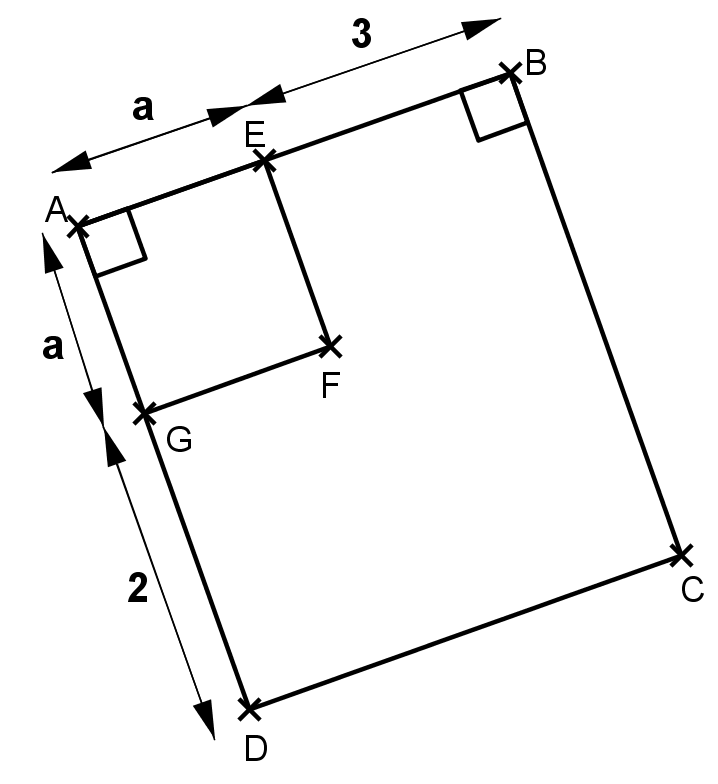
\includegraphics[width=5cm]{images/ex2.png}  
\end{minipage}
\end{tabular}


\bigskip


\textbf{\ul{Exercice 3}} \quad \textit{(2,5 points)} 

\enskip

R�duire l'expression suivante:
A=(3t-6)(-5-t)+4(2t+7)

\bigskip


\textbf{\ul{Exercice 4}} \quad \textit{(3,5 points)} 

\enskip

Pascal ach�te 7 pains au chocoalt et 4 croissants. un croissant co�te $y$
\euro. Un pain au chocolat co�te 0,20 \euro de plus qu'un croissant.

\begin{enumerate}
  \item Exprimer le prix d'un pain au chocolat en fonction de $y$.
  
  \item  Ecrire en fonction de $y$ la d�pense totale de Pascal.
  \item D�velopper et r�duire l'expression trouv�e.
  \item Si un croissant co�te 0,80 \euro, combien doit payer Pascal?
\end{enumerate}


\bigskip

\textbf{\ul{Exercice 5}} \quad \textit{(4 points)} 

\enskip

Dans la figure ci-dessous, le point A appartient au cercle de diam�tre [CT] et
de centre S. Les droites (HS) et (CA) sont perpendiculaires.


\begin{tabular}{cc}
\begin{minipage}{13cm}
\begin{enumerate}
  \item D�monter que les droites (CA) et (AT) sont perpendiculaires.
  \item En d�duire que les droites (HS) et (AT) sont parall�les. Justifier
  votre r�ponse.
  \item D�montrer que H est le milieu du segment [CA].
\end{enumerate}
\end{minipage}
& 
\begin{minipage}{5cm}
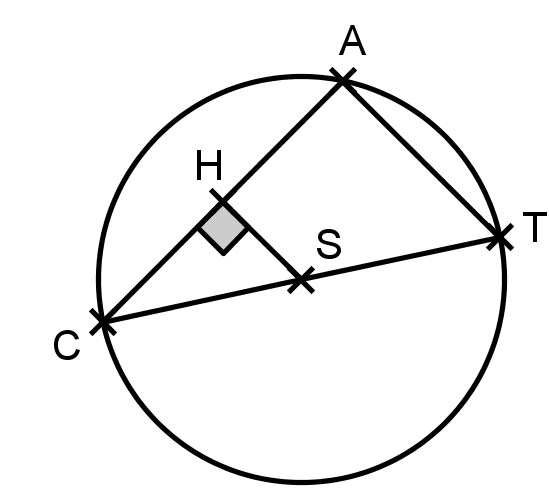
\includegraphics[width=4cm]{images/ex4.png}
\end{minipage}
\end{tabular}

\end{document}
